\subsection{Validazione e collaudo}
\textbf{Periodo}: dal \textbf{2022-03-20} al \textbf{2022-04-07} \mbox{} \\ \mbox{} \\

Le precondizioni sono:
\begin{itemize}
	\item le postcondizioni della fase precedente sono state soddisfatte.
\end{itemize}

Le postcondizioni sono:
\begin{itemize}
	\item aggiornamento e approvazione dei documenti prodotti precedentemente;
	\item esecuzione di tutti i test;
	\item completamento del prodotto software;
	\item realizzazione della presentazione da esporre nella terza revisione, \textit{Customer Acceptance}. 
\end{itemize}

La fase è composta da N \textbf{MANCA} nuove attività:
\begin{itemize}
	\item \textbf{Incremento e verifica dei documenti}: viene aggiornata e migliorata la documentazione;
	\item \textbf{Incremento e verifica delle attività}: se necessario, vengono migliorate le attività di \textit{Technology Baseline} per quanto riguarda la progettazione ad alto livello, la \textit{Product Baseline} riguardo l’aggiunta di design pattern o diagrammi delle classi e di attività e la Codifica formata seguendo l’idea di incrementi ciclici come per la fase precedente. In particolare,  se non ci sono stati ritardi nella codifica si terrà in considerazione l’idea di implementare uno o più casi d’uso opzionali; di conseguenza,  al momento non verranno pianificati gli incrementi in maniera esatta poiché ritenuti troppo prematuri;
	\item \textbf{Validazione e collaudo}: realizzazione degli ultimi test, con successivi controlli finali per verificare se le funzionalità rispettano i risultati attesi,  secondo quanto indicato nel Piando di Qualifica.
\end{itemize}

Questa fase viene suddivisa a sua volta in tre periodi scanditi dalle milestone interne pianificate dal gruppo:
\begin{itemize}
	\item \textbf{primo periodo (dal 2022-03-20 al 2022-03-24))}: in questo primo periodo il gruppo si dedicherà,  se necessario,  a migliorare con oppurtune correzioni i documenti prodotti precedentemente,  inclusi quelli per la \textit{Technology Baseline} e \textit{Product Baseline}.  Inoltre,  si controllerà che i requisiti siano soddisfatti;
	\item \textbf{secondo periodo (dal 2022-03-24 al 2022-04-01)}: nel secondo periodo il team si dedicherà unicamente alla codifica e alla realizzazione dei test;
	\item \textbf{terzo periodo (dal 2022-04-01 al 2022-04-07)}: nell'ultimo periodo,  si incrementeranno i documenti di specifica tecnica e manuale utente,  in base a quanto ulteriormente aggiunto nei periodi precedenti.  Infine,  si verificherà di aver realizzato tutti i test per la validazione e il collaudo,  e si produrrà il materiale necessario da esporre in sede di presentazione del prodotto finale.
\end{itemize}

\begin{figure}[!h]
\centering
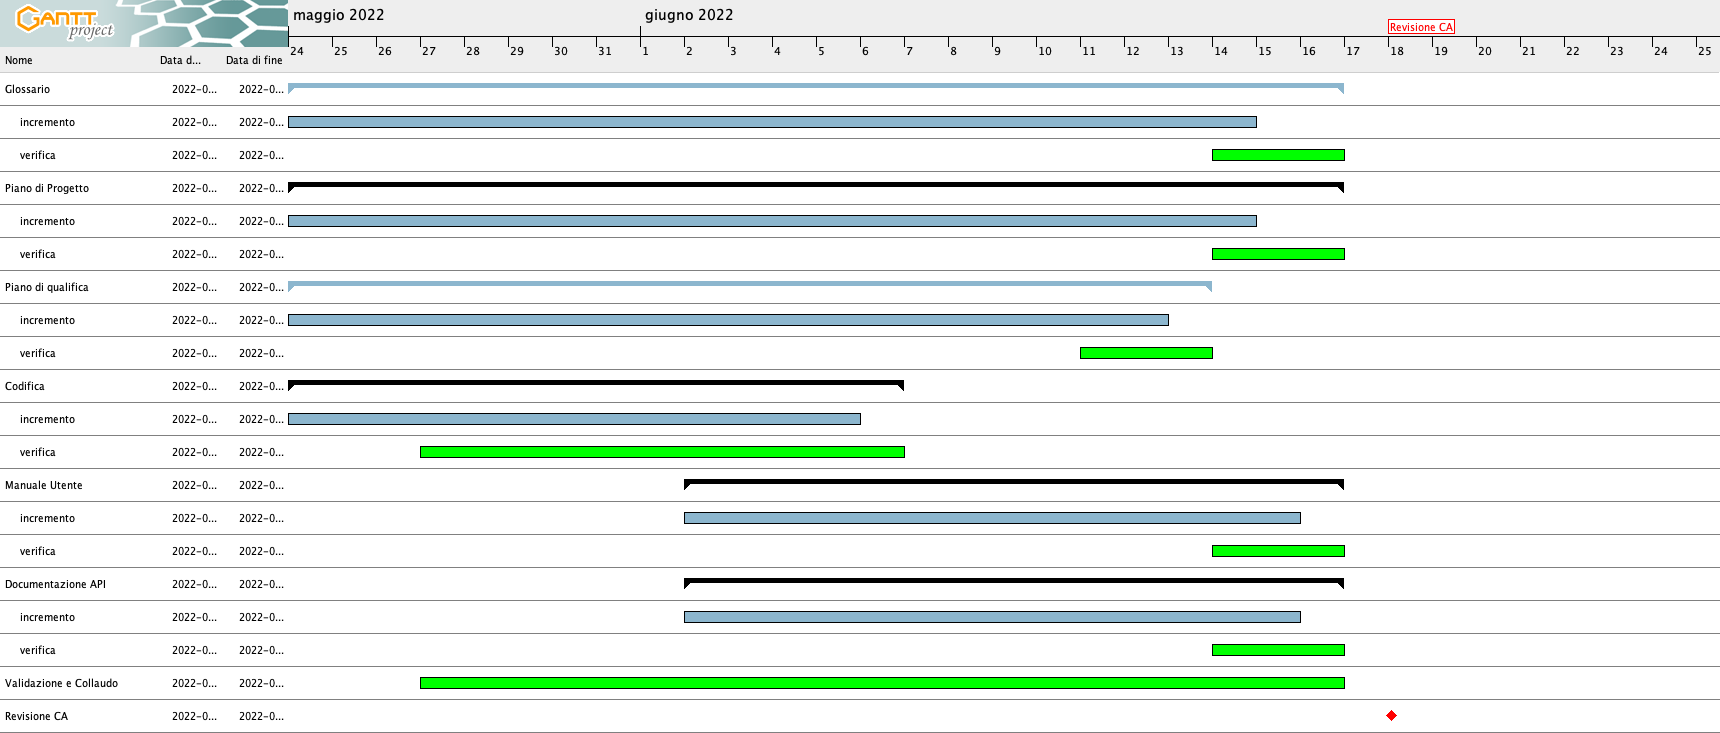
\includegraphics[scale=0.35]{Sezioni/gantt/validazione_collaudo.png}
\caption{Diagramma di Gantt - Validazione e collaudo}
\end{figure}